\documentclass[12pt, a4paper]{report}
\usepackage[top=1cm, left=0.8cm, right=0.8cm]{geometry}

\usepackage[utf8]{inputenc}
\usepackage[russian]{babel}

\usepackage{array}
\newcolumntype{M}[1]{>{\centering\arraybackslash}m{#1}}

\usepackage{hyperref}
\hypersetup{
	colorlinks,
	citecolor=black,
	filecolor=black,
	linkcolor=black,
	urlcolor=black
}

\usepackage{sectsty}
\allsectionsfont{\centering}

\usepackage{indentfirst}
\setlength\parindent{24pt}
 
\usepackage{listings}
\usepackage{xcolor}
\definecolor{codegreen}{rgb}{0,0.6,0}
\definecolor{codegray}{rgb}{0.5,0.5,0.5}
\definecolor{codepurple}{rgb}{0.58,0,0.82}
\definecolor{backcolour}{rgb}{0.95,0.95,0.92}
\lstdefinestyle{mystyle}{
    backgroundcolor=\color{backcolour},
    commentstyle=\color{codegreen},
    keywordstyle=\color{magenta},
    numberstyle=\normalsize\color{codegray},
    stringstyle=\color{codepurple},
    basicstyle=\ttfamily\footnotesize,
    breakatwhitespace=false,
    breaklines=true,
    captionpos=b,
    keepspaces=true,
    numbers=left,
    numbersep=5pt,
    showspaces=false,
    showstringspaces=false,
    showtabs=false,
    tabsize=2
}

\usepackage{graphicx}
\graphicspath{{assets/}}

\begin{document}
	\begin{titlepage}
		\begin{center}
			\large \textbf{Министерство науки и высшего образования Российской Федерации} \\
			\large \textbf{Федеральное государственное бюджетное образовательное учреждение высшего образования} \\
			\large \textbf{«Российский химико-технологический университет имени Д.И. Менделеева»} \\

			\vspace*{4cm}
			\LARGE \textbf{ОТЧЕТ ПО ЛАБОРАТОРНОЙ РАБОТЕ №7}

			\vspace*{4cm}
			\begin{flushright}
				\Large
				\begin{tabular}{>{\raggedleft\arraybackslash}p{8.85cm} p{10.8cm}}
					Выполнил студент группы КС-36: & Золотухин Андрей Александрович \\
					Ссылка на репозиторий: & https://github.com/ \\ 
					& CorgiPuppy/ \\
					& info-sys-admin-labs \\
					Принял: & Митричев Иван Игоревич \\
					Дата сдачи: & 16.04.2025 \\
				\end{tabular}

			\end{flushright}

			\vspace*{6cm}
			\Large \textbf{Москва \\ 2025}
		\end{center}
	\end{titlepage}
	
	\tableofcontents	
	\thispagestyle{empty}
	\newpage

	\pagenumbering{arabic}
	
	\section*{Описание и выполнение задачи}
	\addcontentsline{toc}{section}{Описание и выполнение задачи}	
	\large

	\subsection*{Задание 1}
	\addcontentsline{toc}{subsection}{Задание 1}
	\large
	\begin{center}
		\textbf{Вариант 15}
	\end{center}
	\par
	Написать скрипт \textit{sed}, который заменяет в файле все теги \textit{<div>} на \textit{<p>}, а теги \textit{</div>} удаляет. Протестировать скрипт на различных файлах, показав, что поставленная задача решена верно.
	\lstset{style=mystyle}
	\lstinputlisting[language=Bash]{src/task1/main.sh}
	\lstinputlisting[language=Bash]{src/task1/main.sed}
% \begin{center}
% 	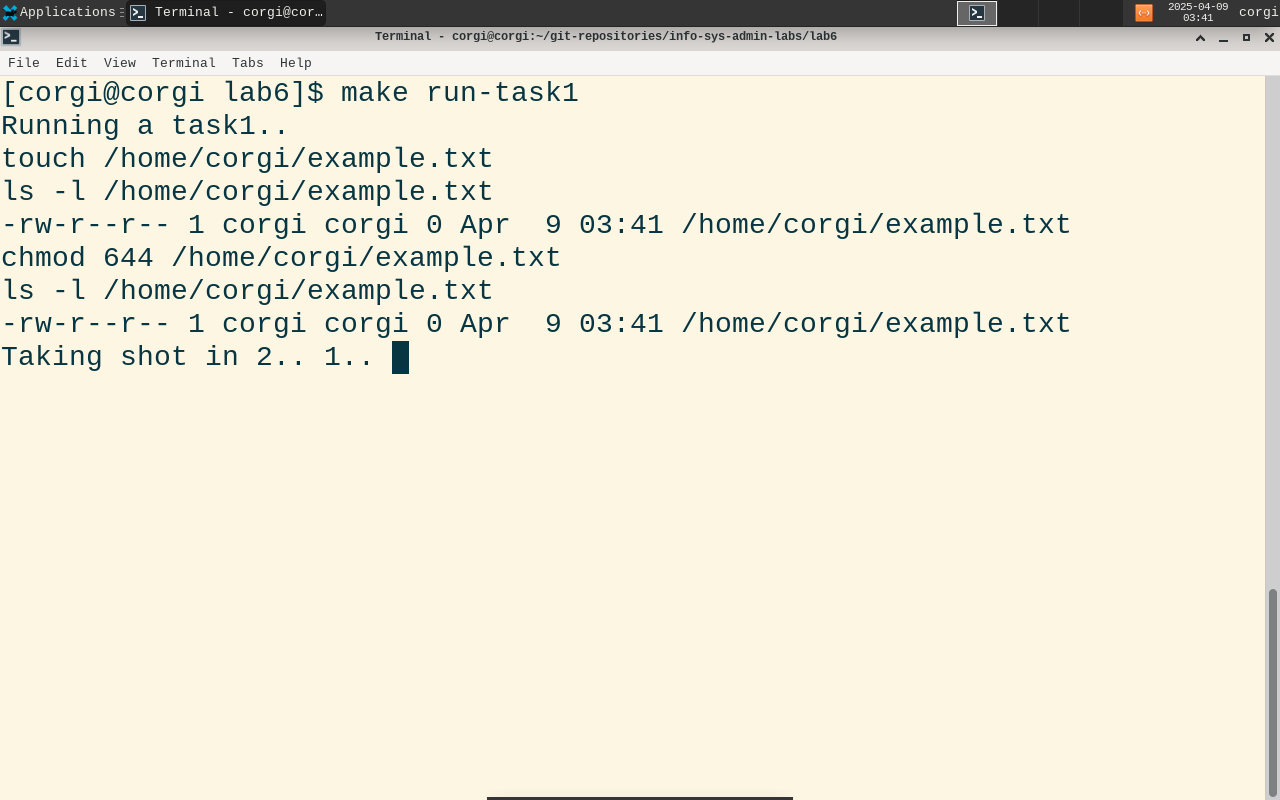
\includegraphics[width=500pt]{task1.png}
% \end{center}

	\subsection*{Задание 2}
	\addcontentsline{toc}{subsection}{Задание 2}
	\large
	\begin{center}
		\textbf{Вариант 32}
	\end{center}
	\par
	Содержимое файла \textit{atoms.xyz}
	\begin{center}
		\begin{tabular}{||c|c|c|c||}
			\hline
			Atom & X & Y & Z \\

			\hline
			Ir & 0.99437992990524 & -0.34269845108108 & -3.09726116046547 \\

			\hline
			C & -1.78523435834955 & -0.80128428317708 & -6.59331044461245 \\

			\hline
			C & -3.31598719563957 & -0.92733718351966 & -6.50054352181805 \\

			\hline
			C & -1.40950141330235 & 0.64386728136198  &	-6.98255100716577 \\

			\hline
			O & -1.16164771974228 & -1.22773178801588 &	-5.44314154793957 \\

			\hline
			H & -1.49733129676448 & -1.42721354486802 & -7.48249131009368 \\

			\hline
			H & -3.59159398532618 & -1.96049032471667 & -6.27578865140234 \\

			\hline
			H & -3.68778595322297 & -0.29518726167605 & -5.68835685788211 \\

			\hline
			H & -3.81524644395587 & -0.62800602683343 & -7.42846940234560 \\

			\hline
			H & -0.32436472113108 & 0.76472964945055  & -7.02744643337563 \\

			\hline
			H & -1.82844016240678 & 0.92188046399308  & -7.95536084618941 \\

			\hline
			H & -1.77902163220926 & 1.34747072213403  & -6.23401704120998 \\

			\hline
			K & 1.07103536196612  &	-1.81284456700227 &	-6.52587649854301 \\

			\hline
		\end{tabular}
	\end{center}
	\par
	С помощью \textit{awk} обработать исходный файл \textit{atoms.xyz} в соответствии с заданием. Итоговые переменные/файл вывести на экран.
	\par
	Считать вещественное число с консоли (с помощью \textit{read}) и заменить этим числом все значения координаты \textit{Y}, меньшие \underline{0}, в исходном файле.
	\lstset{style=mystyle}
	\lstinputlisting[language=Bash]{src/task2/main.sh}
	\lstinputlisting[language=Bash]{src/task2/main.awk}
% \begin{center}
% 	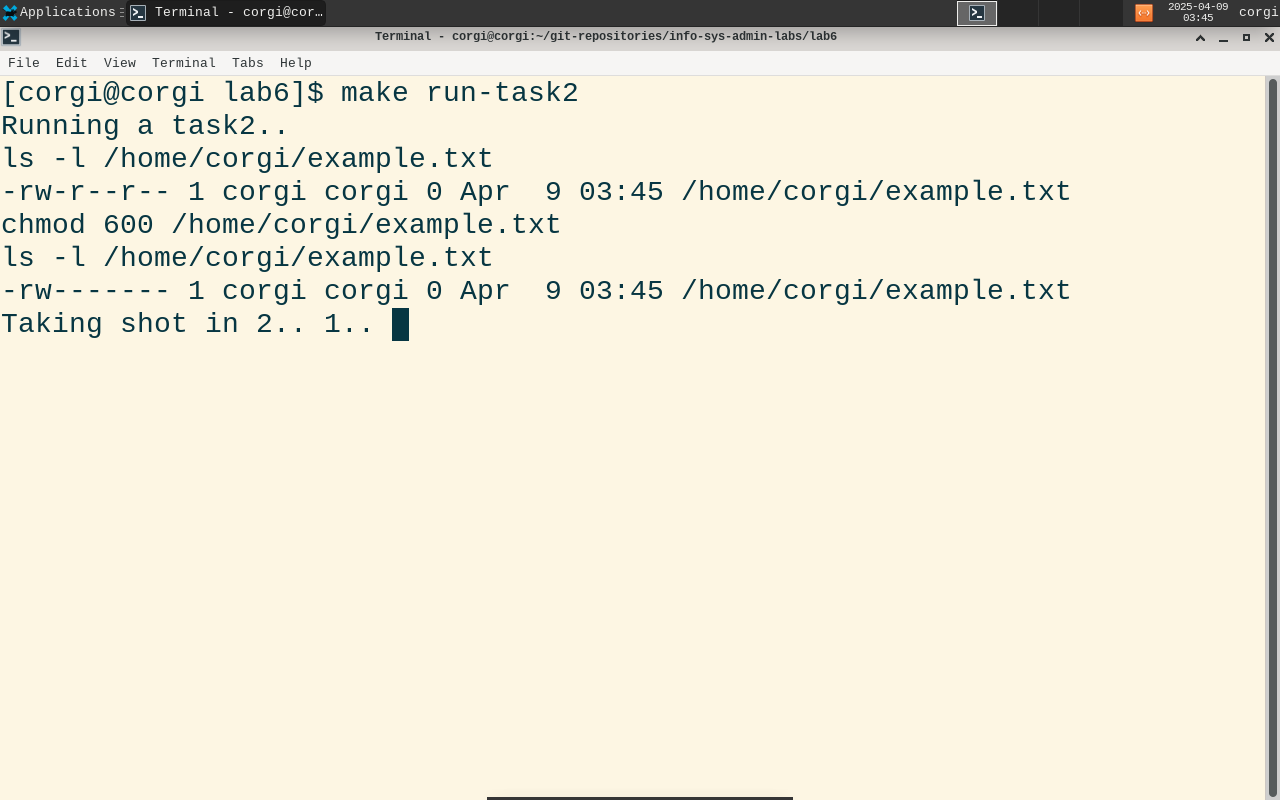
\includegraphics[width=500pt]{task2.png}
% \end{center}

	\subsection*{Задание 3}
	\addcontentsline{toc}{subsection}{Задание 3}
	\large
	\begin{center}
		\textbf{Вариант 49}
	\end{center}
	Напишите калькулятор на \textit{awk}, умеющий выполнять четыре основных арифметических действия для всех примеров, введённых в файл. В примерах операнды вводятся через пробел, в одной строке - один пример, например, \underline{3.29 + 5.28}.
	\par
	\lstset{style=mystyle}
	\lstinputlisting[language=Bash]{src/task3/main.sh}
	\lstinputlisting[language=Bash]{src/task3/main.awk}
	\lstinputlisting[language=Bash]{src/task3/random.awk}
\end{document}
